\section{Scanning CT}

\subsection{CT and HU values}
%% see link: https://web.archive.org/web/20070926231241/http://www.intl.elsevierhealth.com/e-books/pdf/940.pdf
Computed Tomography (CT) scan leverages X-rays to generate images of the body through rapid rotation of the X-ray tube. Then \textbf{attenuation value} of the tissue can be calculated from the intensity reading of the tissue of each voxel to reconstruct the pixels in the images.\\

\subsubsection{Attenuation Value}
Given a photon's initial intensity $I_{0}$, the attenuation value (or Absortion coefficient) $\mu$ is the coefficient describing the change of $I_{0}$ after it pass through an object. An illustration is shown in figure \ref{fig:attenutation}. In linear case with spacial parameter $x$. The new intensity can be denote as: $$I(x)=I_{0} e^{-\mu x}$$ In the non-linear case, the non uniform absorbtion is described as: $$\frac{d I(x)}{d x}=-\mu(x) I(x)$$ 
Then we write the new intensity as: $$I_{non-linear}(x)=I_{0} e^{-\int_{a}^{b} \mu(x) d x}$$

\begin{figure}[h]
	\centering
	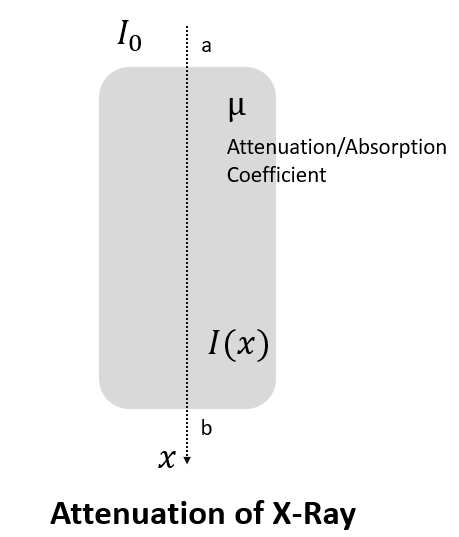
\includegraphics[width=0.4\textwidth]{img/background_img/attenutation}
	\caption{Attenuation}
	\label{fig:attenutation}
\end{figure}

\subsubsection{Hounsfield Units}
Hounsfield units (HU) represents the average attenuation value of each voxel compared to the attenuation value of water. CT numbers can take value between -1000 and 1000 while 2000 shades of grey is out of the capacity of human eyes can distinguish. Thus, only a limited number of HU are displayed for human interpretation. Lung window is normally set to [-1250, 250]. Figure \ref{fig:HU_value} shows some common HU value range of different matters.
\begin{figure}[h]
	\centering
	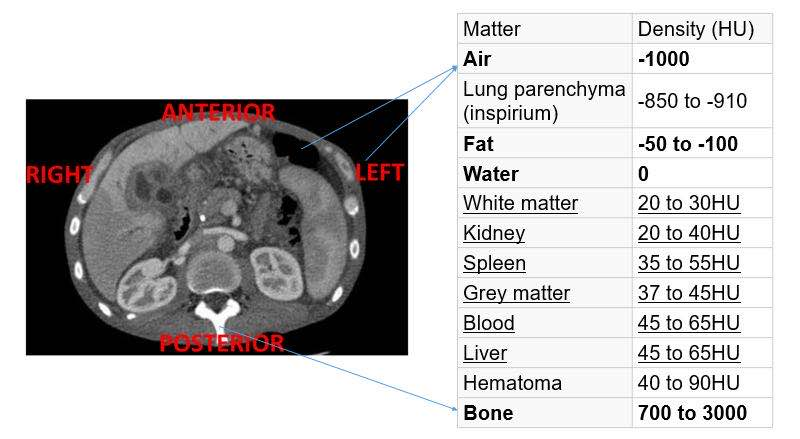
\includegraphics[width=0.8\textwidth]{img/background_img/HU_value.png}
	\caption{Common Hounsfield Unit values including human body tissue}
	\label{fig:HU_value}
\end{figure}

\subsection{Thick and thin slices}
Thin slices are generally regarded as planes representing thickness of less than 3mm \footnote{http://tech.snmjournals.org/content/36/2/57} In our work, we experienced slice thickness from 1mm to 8mm. \\
{\color{red} In medical CT scanning, considering the dose of CT, and the equipment limitation, thick slice tend to show little or no slice-wise information along the axial slices.} An illustration of thick and thin slice difference is shown in figure \ref{fig:thick_thin_slice}

\begin{figure}[h]
	\centering
	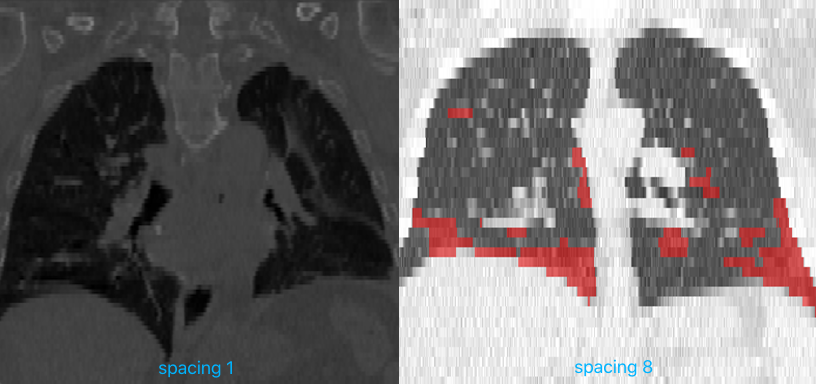
\includegraphics[width=0.8\textwidth]{img/background_img/thin_thick_slice.png}
	\caption{Spacing diversity along the Z (Axial) axis. Left: thin slice with spacing 1; Right: thick slice with spacing 8.}
	\label{fig:thick_thin_slice}
\end{figure}
\newpage

\section{Deep learning fundamentals}
In this section, we briefly mention some of the fundamentals of Deep Learning and some layer structures used in our experiment, note that most of our notation follows the book \textit{Deep Learning}\cite{Goodfellow-et-al-2016}.

\subsection{Optimization in training neural network}
%TODO mention optimizers here
\subsubsection{Gradient Descent}
Fist of all, Gradient Descent Algorithm leverages the first order derivative to modify the weights so that a function gradually reach its local minima. The mathematical definition is:
$$\boldsymbol{\theta}=\boldsymbol{\theta}-\boldsymbol{\alpha} \cdot \nabla \mathrm{J}(\boldsymbol{\theta})$$ 
in which $\mathrm{J}$ denotes the loss function, $\theta$ is the trainable parameter and $\alpha$ is the learning rate. 
\subsubsection{Adam optimizer}

%TODO adam optimization
\subsection{Convolutional Neural Network}
%TODO provide a brief theoretical summary of Convolution here
Convolutional neural networks (CNN) improved deep learning with respect to \textbf{Sparse interactions, parameter sharing and equivariant representations} that employ mathematical convolution operation denoted with asterisk symbol $*$. The imaging domain usually make use of discrete convolution: $$s(t)=(x * w)(t)=\sum_{a=-\infty}^{\infty} x(a) w(t-a)$$
We here clarify that in our following notation, we call $x$ the \textbf{input}, $w$ \textbf{kernel} or \textbf{weight}, and $s$ \textbf{output} or \textbf{feature map}.\\
In two dimensional case:
$$S(i, j)=(I * K)(i, j)=\sum_{m} \sum_{n} I(m, n) K(i-m, j-n)$$
\subsection{Activation function}
Activation function $\phi$ (usually non-linear) introduce non-linearity into neural networks.
In modern Neural Networks, some of the activation functions are:
\begin{itemize}
	\item Recitified Linear Unit (RelU): $\sigma(x)=\max (0, x)$
	\item Eponential Linear Unit (Elu): $\sigma(x)=\left\{\begin{array}{ll}\alpha\left(e^{x}-1\right) & \text { for } x<0 \\ x & \text { for } x \geq 0\end{array} \mid \alpha \geq 0\right.$
	\item Leaky Relu: $\sigma(x)=\left\{\begin{array}{ll}0.01 x & \text { for } x<0 \\ x & \text { for } x \geq 0\end{array}\right.$
	\item Sigmoid: $\sigma(x)=\frac{1}{1+e^{-x}}$
	\item Softmax: $\sigma(\boldsymbol{x})_{i}=\frac{e^{x_{i}}}{\sum_{j=1}^{n} e^{x_{j}}} \mid i \in\{1, \ldots, n\}$ Softmax scale the layer output between 0 and 1 and its sum = 1.
\end{itemize}

\begin{figure}[h]
	\centering
	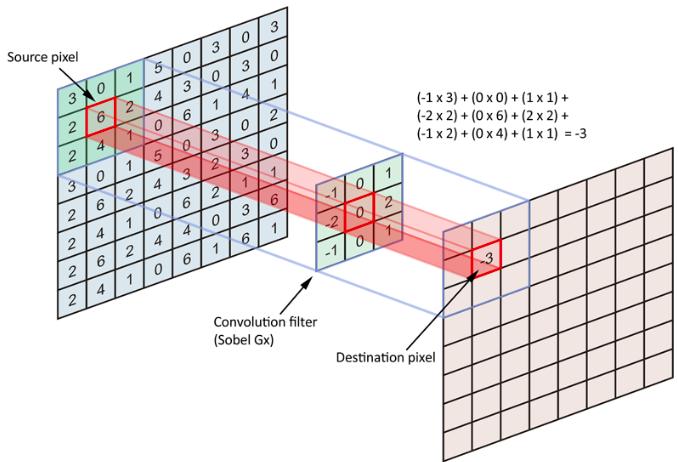
\includegraphics[width=0.8\textwidth]{img/background_img/convolution}
	\caption{An example of convolution using Sobel filter} 
	%TODO change citation \footnote{https://medium.com/pallawi.ds/ai-starter-build-your-first-convolution-neural-network-in-keras-from-scratch-to-perform-a059eaa6d4ff}
	\label{fig:convolution}
\end{figure}

\subsection{Pooling}
Pooling function modify the output of a layer at a specific location through summarizing its neighboring outputs that helps an approximate invariant. Max pooling is simply the maximum output within a neighborhood. Average pooling takes the average of the neighborhood as output instead of the maximum. An illustration of pooling is shown in figure \ref{fig:pooling}
\footnote{https://link.springer.com/article/10.1007/s00521-019-04296-5/figures/1}
\begin{figure}[h]
	\centering
	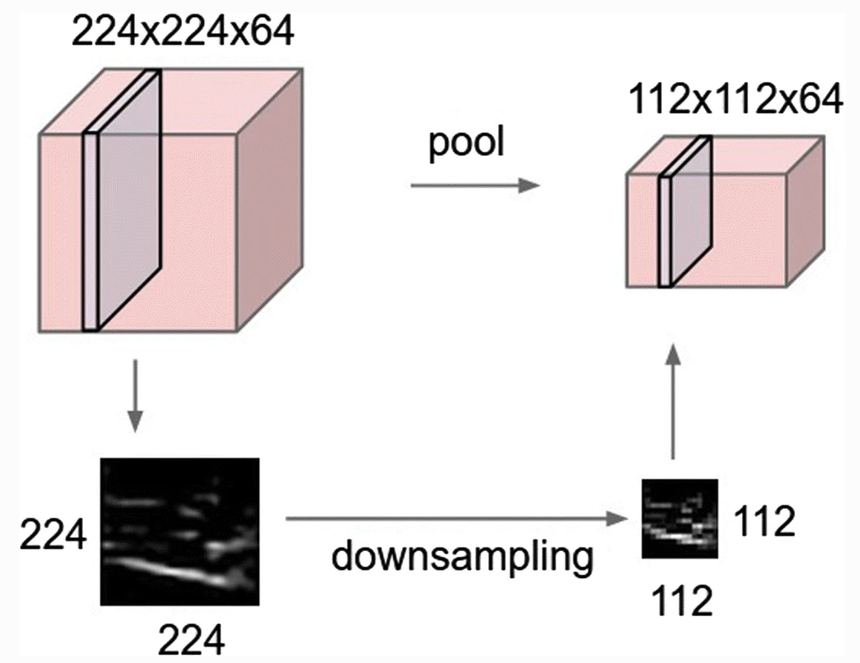
\includegraphics[width=0.6\textwidth]{img/background_img/pooling_img}
	\caption{Downsampling using pooling}
	\label{fig:pooling}
\end{figure}

\subsection{Batch Normalization}
Batch normalization (BN) was proposed in \cite{BatchNorm} to mitigate \textbf{internal covariate shift} by fixing the mean and variance of each layer's inputs so that it allows each layer of the network to learn more independently from the rest of the layers.\\

Batch Normalization adds two trainable parameters to each of the layer. The process of BN is shown below:
\begin{algorithm}
    \caption{Batch Normalisation}\label{BatchNorm}
    \hspace*{\algorithmicindent} \textbf{Input:} Values x over a mini-batch: $Batch = {x_{1...m}}$, $\gamma$, $\beta$\\
    \hspace*{\algorithmicindent} \textbf{Output:} $BN_{\gamma,\beta}(x_{1...m})$
    \begin{algorithmic}[]
    \State $\mu_{\mathcal{B}} \gets \frac{1}{m} \sum_{i=1}^{m} x_{i}$    
    \State $\sigma_{\mathcal{B}}^{2} \leftarrow \frac{1}{m} \sum_{i=1}^{m}\left(x_{i}-\mu_{\mathcal{B}}\right)^{2}$
    \State \Comment{Normalizing}
    \State $\widehat{x}_{i} \leftarrow \frac{x_{i}-\mu_{\mathcal{B}}}{\sqrt{\sigma_{\mathcal{B}}^{2}+\epsilon}}$  
    \State \Comment{Scale and shift}
    \State $y_{i} \leftarrow \gamma \widehat{x}_{i}+\beta \equiv \mathrm{B} \mathrm{N}_{\gamma, \beta}\left(x_{i}\right)$
    \end{algorithmic}
    \end{algorithm}

%TODO add more bullshit about batch normalization

\subsection{Attention Gate}
%TODO add details of the impelemted attention gate to the network
Attention Gate proposed in \cite{Attention_gate_network} provided a way that we can train the network for segmentation with extra localization objective.
Let $\mathbf{x}^{l}=\left\{\mathbf{x}_{i}^{l}\right\}_{i=1}^{n}$ denotes the activation map over a layer such that $x_{i}^{l}$ is the pixel-wise feature vector with dimension equals to the number of feature maps of the output. Attention Gate learn a scaling vector $\alpha_{i}^{l}$ as the weight to scale the feature vector, more formally:
$$\hat{\mathbf{x}}^{l}=\left\{\alpha_{i}^{l} \mathbf{x}_{i}^{l}\right\}_{i=1}^{n}$$
The additive attention in the paper, can then be written as:
$$q_{a t t, i}^{l}=\psi^{T}\left(\sigma_{1}\left(\boldsymbol{W}_{x}^{T} \boldsymbol{x}_{i}^{l}+\boldsymbol{W}_{g}^{T} \boldsymbol{g}+\boldsymbol{b}_{x g}\right)\right)+b_{\psi}$$
$$\alpha^{l}=\sigma_{2}\left(q_{a t t}^{l}\left(\boldsymbol{x}^{l}, \boldsymbol{g} ; \boldsymbol{\Theta}_{a t t}\right)\right)$$
in which $\sigma_{1}$ denotes a non-linear activation function such as ReLU and $\sigma_{2}$ is a normalizing function so that $\sum_{i} e^{q_{a t t, i}^{l}} = 1$. In the paper, the author used sigmoid as activation function. Note the the attention gate is usually obtained from a coarser feature map. Figure \ref{fig:att_gate} shows the attention gate structure.

\begin{figure}
\centering
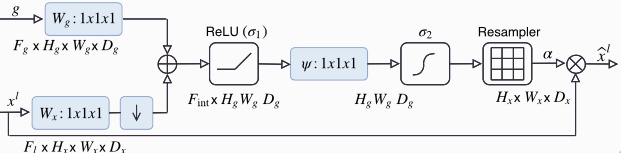
\includegraphics[width = 0.8\textwidth]{img/background_img/attention_gate}
\caption{Attention Gate structure proposed in \cite{Attention_gate_network}}
\label{fig:att_gate}
\end{figure}


\subsection{Encoder-Decoder architecture}
One of the breakthrough in both medical and non-medical segmentation is the presense of an Encoder-Decoder architecture network. Encoder combines non-linear feature extracting with convolution and down-sampling so that the Encoder can learn a rather 'rich hidden space representation'. The Decoder generates segmentation through upsamle or transpose convolution so that the network ouput is the same dimension of the input images. Paper \cite{Liu2018DeepCN} leveraged the Encoder-Decoder to segment bones in MR images. Figure \ref{fig:segnet_encoderdecoder} shows the encoder-decoder architecture leveraged in the paper.

\begin{figure}
\centering
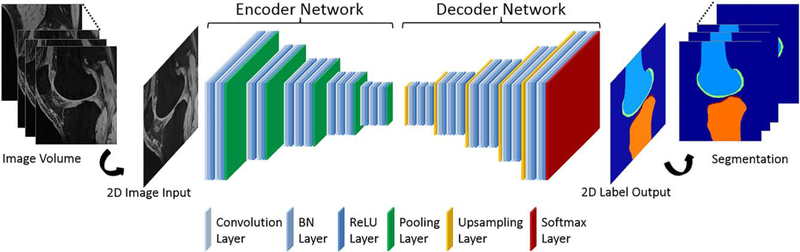
\includegraphics[width = 0.9\textwidth]{img/background_img/segnet_background}
\caption{An Encoder-Decoder structure network proposed in \cite{Liu2018DeepCN}}
\label{fig:segnet_encoderdecoder}
\end{figure}


\subsection{U-Net and skip connections}
This section we introduce several well known methods in medical segmentation. Unet \cite{ronneberger_u-net_2015} and its variations plays a dominant role in current medical segmentation tasks, and it is often used as a baseline model for performance evaluation in the literature.\\

U-Net \cite{ronneberger_u-net_2015} is among one of the most widely used medical segmentation models since the day it was proposed based on the Encoder-Decoder network structure it proposed. The original Unet consists of a contracting path followed by an expansive path that gives a "U" shaped architecture. The network architecture is shown in figure \ref{fig:unet-arch}.
Later this 2D model was extended to 3D version in \cite{ourselin_3d_2016} for for Kidney segmentation tasks so that the model learn features from information implicated between slices.\\
\begin{figure}
\centering
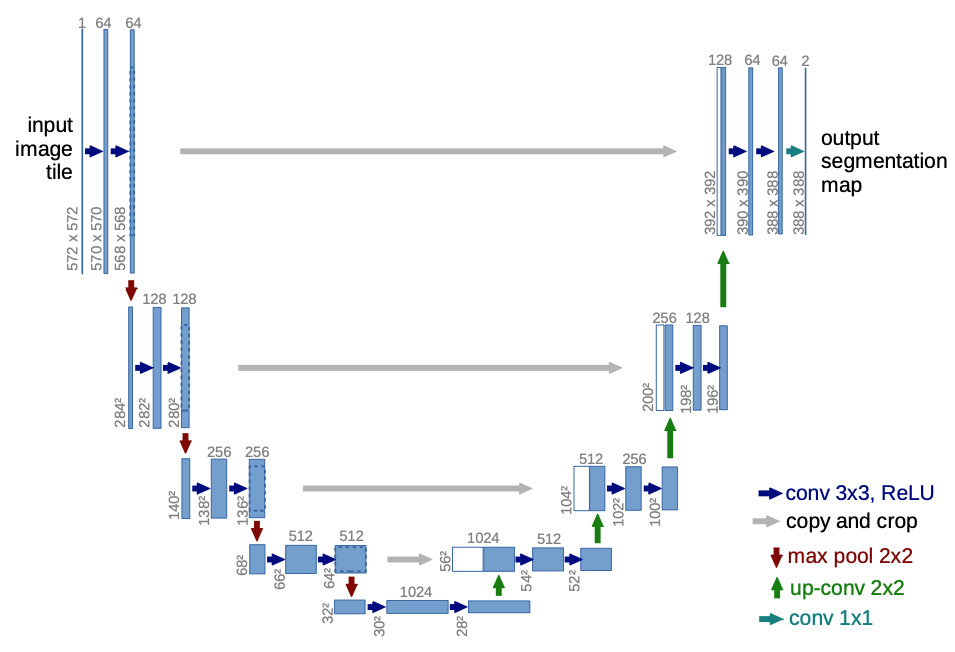
\includegraphics[width = 0.8\textwidth]{img/Unet_architecture}
\caption{Original Unet architecture in \cite{ronneberger_u-net_2015}}
\label{fig:unet-arch}
\end{figure}

VNet \cite{milletari_v-net_2016} is another 3D variation of Unet, and the network performed evaluation on prostate dataset. Each block of convolution has a residual feature that the input of the block is added to the last convolutional layer. The author argued that leverage residual structure enables network convergence in a fraction of the amount of time other network used.


\section{Small Sample Segmentation}

\subsection{Data augmentation}
In medical domain, huge dataset consists of large numbers of carefully labelled samples is rarely available due to heavy workload for annotations, rarity of disease, ethic issues of data acquire process and data privacy. Furthermore, different data acquire protocols (i.e. CT machines used by different hospitals) brings difficulties to clinical practice for good accuracy of existing pre-trained models. As a result, few shot learning and/or few shot segmentation has been explored in recent years. 
In this section, we focus on a few approaches that has been used in current literature which aim to explore the potential of existing training samples through various augmentation methods to alleviate the insufficient training samples in medical imaging. We discuss data augmentation method as well as the amount of data used in each work. Table \ref{tab:Augtable} provide an overview of each method.

\subsection{Traditional Data Augmentation}
Traditional Data augmentation methods in imaging domain refers to the process that does not require such training data to learn a transformation.\\

Paper \cite{zhang_when_2019} investigated data augmentation methods under 3D medical domain of MR and ultrasound images. 
The data augmentation process consists of a sequence of traditional transformation techniques. The paper argued that sharpness in medical images during training process limits model generalization thus applying gaussian filter to images take noise into consideration. Brightness and contrast difference caused by variations in scanning protocols brings potential domain shift thus a sequenced random shift followed gamma correction and random linear transform in intensity are reasonable data augmentation methods. Finally spatial transformations including rotation, flipping, scaling and deformation is added to the augmentation process.

The source domain in this method is Prostate dataset \footnote{http://medicaldecathlon.com/index.html\#tasks} which consists 48 4D volumes.
We argue here that the stacked transformation is a physical transformation process independent to the size of dataset because no learning or training process is required in this augmentation method thus might bring benefits to our task. However, although Deep learning models (Convolutional Neural Networks) are scale and rotation invariant, medical images differs from natrual images that scanning was conducted with a certain position, i.e. patients usually lie on a CT bed facing up for CT scanning. Thus flipping the lung volumes or rotating the lungs more than 5 degrees is less reasonble.\\


%%%---------
Another method "mixup" by \cite{zhang_mixup_2018} based on generic vicinal distribution, which generates new samples through interpolation between two existing data. The author argued that this method works as a regularizer which encourages linear behavior between training samples. In terms of imaging, the augmentation is applied to CIFAR 10 (2D non medical) Dataset. The calculation method in paper follows the following equations where $x_{i}$ and $x_{j}$ are training examples and $\lambda$ is usually sampled from beta distribution.
$$\tilde{x}=\lambda x_{i}+(1-\lambda) x_{j}$$
$$\tilde{y}=\lambda y_{i}+(1-\lambda) y_{j}$$
The work was originally implemented on training GANs. Later in medical domain, \cite{panfilov_improving_2019} further investigated mixup method on Knee MR images on OIA database \footnote{http://www.oai.ucsf/.edu/} that consists of 88 3D MRI scans. The work showed mixup improves generalization under their experiment setup while having risk of slight underfitting due to to the strong regularization. The author further mentioned not using weight decay in the experiment solve the underfitting issue.
\cite{tajbakhsh_embracing_2020} summarized mixup augmentation method gives "soft labels". Variations of the mixup method utilize asymmetric is further explored in \cite{li_overfitting_2019} trained on Brain MR images, and the method reports huge gain under their experiment setup.

\subsection{Learning for augmentation}
Following the traditional augmentation methods, we here want to discuss a few medical image augmentation based on deep learning. Specifically we focus on those who used one or a few data during the augmentation so that it follows the small sample segmentation setup.\\

%TODO citation in adversarial defense
Adversarial defense was deployed in \cite{suk_brain_2019} for the augmentation of small samples in Brain MR segmentation. Adversarial samples generated though Fast Gradient Sign Method\cite{goodfellow_explaining_2015} and then added as training data to improve the robustness. Paper in \cite{chen_one-shot_2020} leverage paired MRI-CT data to construct a cycle-GAN model that convert an given MRI to a CT style image to segment Craniomaxillofacial Bone structure.\\

\begin{table}
\begin{tabular}{lllll}
\hline
Paper                                             & Method                        & Dataset              & Number of samples &  \\
\hline
\cite{zhang_when_2019}       & Stacked traditional transform & Prostate dataset     & 48 4D volumes     &  \\
\cite{zhang_mixup_2018}       & mixup                         & CIFAR 10             & Huge              &  \\
\cite{panfilov_improving_2019} & mixup                         & Knee MR images       & 88 3D MRI         &  \\
\cite{li_overfitting_2019}   & Asymmetric mixup              & BraTS               &  not specified             &  \\
\cite{suk_brain_2019}                    & Adversarial defense           & MRBrainS18 challenge & 7 train, 14 test  &  \\
\cite{chen_one-shot_2020} &  Cycle GAN &  Brain CT and MR&1 MRI-CT pair; Large MRI\\
\hline
\end{tabular}
\caption{Data Augmentation methods}
\label{tab:Augtable}
\end{table}

\subsection{Transfer Learning}
In medical domain, few shot learning mainly focus on transfer learning from pre-trained networks that leverage both medical and non-medical datasets.\\

%Although recent machine learning community have seen a growing number of medical segmentation public dataset available, the amount of data samples is still less desirable compared to natural, non-medical datasets. Thus researchers have seek for methods that leverage natural images.\\

In Lung CT segmentation area, Sports-1M dataset has been used as source domain to train a multi-task learning model for nodule malignancy prediction and rating \cite{hussein_risk_2017}. The author reported significant improvement in the prediction accuracy, however, did not mention the proportion of data used for transfer training.\\

People tend to choose datasets from closer domain for transfer learning. It is reasonable to consider methods that transfer across disease in the same structure under the same modality. In our case, we might want to investigate transfer learning from NSCLC Dataset to Covid segmentation set given that both of them are lung CT scans.\\

Recent work explored several across disease transfer learning training techniques under MRI domain \cite{wang_improving_2019}. The paper evaluated three transfer learning methods trained on 3D U-Net by Fine tuning the last three layers, Fine tuning the decoder and Fine tuning all model parameters. 
The Source Dataset: Multiple Sclerosis Dataset consists 3630 MRI volumes and used Brain Tumor Dataset as Target dataset including 210 high-grade glioma (HGG) and 75 low-grade glioma (LGG) Brain MRI scans. The training target is a decaying weighted categorical cross entropy loss weighted by relative voxel. Their best validation performance of pre-trained network achieved validation performance AUC 0.77. Experiment result on 20, 50, 100 and 150 samples during Fine tuning respectively showed that Fine tuning all parameters out performed the rest methods in most cases.\\

One potential drawback is that compared to the our task, the target training set is relatively larger, the performance is expected to be less ideal when using "fine tune all" method using 4 or less volumes in our case.

\subsection{Special network design}
Transfer learning methods usually require small samples to update millions of parameters that take the risk of overfitting \cite{shaban_one-shot_2017}. The design of multiple branch network, usually includes conditioner arm and segmentation arms inspired the deep learning in medical domain to go beyond transfer learning while encourage a stronger between-arms interaction to compensate the lacking in pre-trained model \cite{roy_squeeze_2019}. The proposed method perform 3D volume segmentation at test time while use 2D images during training. However the method requires start and end slice to be indicated for each query volume and still not achieving good dice score.\\

Paper \cite{suk_brain_2019} trained segmentation of Brain MR image on 7 brain volumes after Adversarial defense augmentation. The work first split the segmentation from easy to hard into 2 individual classifiers then joint learning with dense pixel segmentation. The author reported that the result outperformed Unet and Vnet method trained from scratch. We argue that the augmentation provide good result in the segmentation accuracy while the segmentation part is not well explained in the paper. We have emailed the author for further details.

% TODO change citation in table header
\begin{table}
\begin{tabular}{p{1cm} p{5cm} p{4cm} p{4cm}}
\hline
Paper    & Method                                & Domain Details                                          & Task                                       \\
\hline
{\cite{shaban_one-shot_2017}} & Design Conditional Branch             & Target PASCAL-5        & Few shot segmentation                      \\
{\cite{rakelly_few-shot_nodate}} & Guidance network                      & Target PASCAL VOC             & Few shot segmentation                      \\
{\cite{hussein_risk_2017}} & Non medical to medical transfer       & Source: Sports-1M;  Target: Lung nodule                  & Multi-task learning: prediction and rating \\
{\cite{wang_improving_2019}} & Across domain transfer                & Source: MSD; Target: Brain Tumor Dataset & Segmentation                               \\
{\cite{shaban_one-shot_2017}} & Augmentation+pixel dense segmentation & Only trained on 7 brain Volumes                         & Dense segmentation                         \\
{\cite{suk_brain_2019}}  & Branch network design                 & --                                                      & Segmentation                               \\
\hline
\end{tabular}
\caption{Small sample methods in medical and non-medical domain}
\label{tab:small sample learning}
\end{table}	

\subsection{Learning with unlabelled data}
Another common scenario with medical imaging is that, a small set of labelled annotations is available and a relatively larger set of data was collected but not labelled. In this section, we briefly mention three types of work that leverage unlabelled data: training encoder, noise removing, and semi-supervise learning. Both training encoder and noise removing serves as a pretrained network that are usually fined-tuned using the methods we described in the previous section. Semi-supervise learning was proposed to further make use of the unlabeled samples to guide the network update more directly throughout the training process.

\subsubsection{Training encoder as initialization}
Training encoder part without expert labeling usually make use of spatial information of the image such as slice order \cite{10.1007/978-3-319-66179-7_47} and direction \cite{8759553}. \\

In the work \cite{8759553}, authors trained a network to predict a transformation of orientation by rotating or flipping the input slice, and then fine tune the network to classify retinal imaged of diabetes patients. One potential use of this type of initialzation for segmentation task is that we can append the Up-Convolution then transfer on segmentation labels.\\

Paper \cite{10.1007/978-3-319-66179-7_47} trained a encoder that, given a reference slice and a prediction slice, predict the prediction slice is above of behind the reference slide so that the network can learn spatial information using the unlabelled images.\\

\subsubsection{Noise removing}
Instead of training a surrogate task such as training encoder leveraging spatial or location information as a pretraining task, Zongwei Zhou \cite{zhou_models_2019} provided another probability for pretraining both encoder and decoder that used together can serve as weight initialization for a segmentation model, and encoder used on its own is a pretrained feauture extractor for classification task.\\

The work trained a Unet-style network that given a randomly cropped and sliced image, first destroy the image through a sequence of random non-linear transformation, local shifting, out/in-painting then forward the image to restore the original image by minimizing the mean-square-error during training. The author argue that in that way, both the generalizability and the detail feature encoding can be learnt which can be leveraged in later transfer learning process. Figure \ref{fig:genesis-net} showed the restoration process. The model was trained on Lung CT images which is close to our task while the provided model was in 3D version, later in the experiment stage, we actually flattened the pretrained weight into 2D for future training.

\begin{figure}
	\centering
	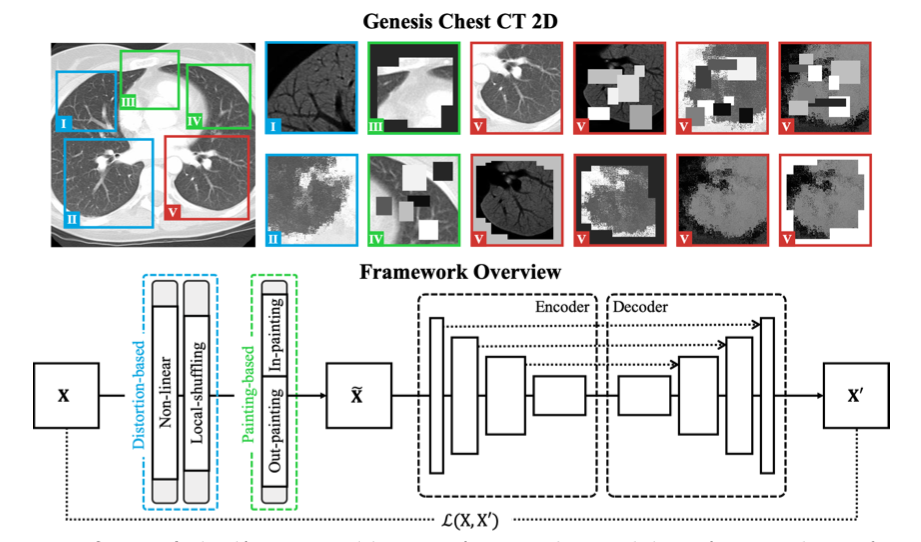
\includegraphics[width=0.8\textwidth]{img/background_img/Genesis_illustration.png}
	\caption{An illustration of Model Genesis pre-training (Figure from the original paper \cite{zhou_models_2019})}
	\label{fig:genesis-net}
\end{figure}

\subsubsection{Semi-supervise}
Semi supervise approach usually add a prediction consistency loss during training. \cite{tarvainen_mean_2018} propsed a teacher-student training strategt such that two networks are train together. The proposed so called 'Mean-teacher' network trained two network simultaneusly. The network design consists of two isomorphic networks that serves as teacher and student. In the beginning of the semi-supervise training, a copy of the teacher model is also created called the student network. For expert-labelled samples, the student model was update using the prediction loss.
Now given a new set of unlabelled raw images, the student network are trained using the prediction consistency cost between student and teacher model. The teacher model weights are updated periodically using an exponential moving average of the student network instead of back propogate the loss directly. Figure \ref{fig:mean-teacher} explains the training process. \\

We here further gives the defnition in the original work \cite{tarvainen_mean_2018}. More formally, define the consistency of the prediction as:
$$J(\theta)=\mathbb{E}_{x, \eta^{\prime}, \eta}\left[\left\|f\left(x, \theta^{\prime}, \eta^{\prime}\right)-f(x, \theta, \eta)\right\|^{2}\right]$$
where x is the input data (image), $\theta, \eta$ denotes the weight and noise in the teacher model and $\theta', \eta'$ denotes the weight and noise in the student model.
The weight update in the teacher model can then be written as:
$$\theta_{t}^{\prime}=\alpha \theta_{t-1}^{\prime}+(1-\alpha) \theta_{t}$$ in which $\alpha$ is the smoothing parameter showing how much the teacher want to move given the new student network.\\

\begin{figure}
	\centering
	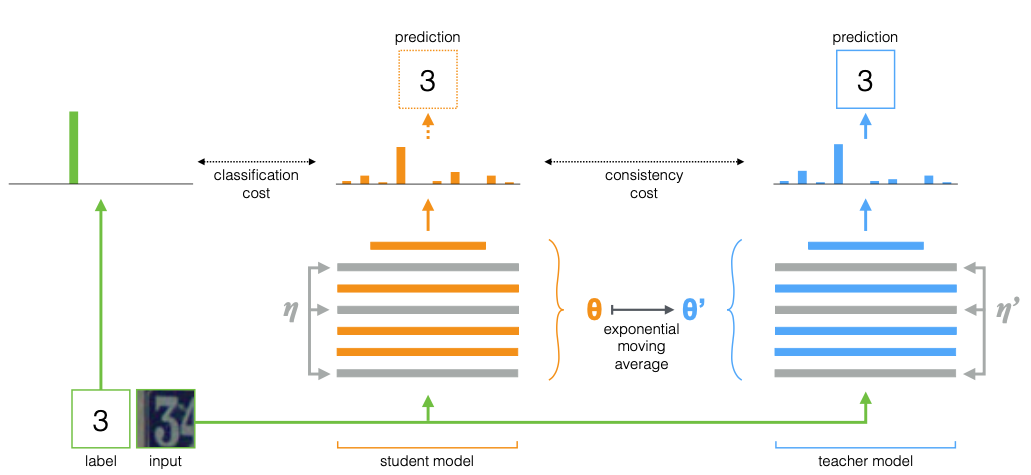
\includegraphics[width=0.8\textwidth]{img/background_img/mean-teacher.png}
	\caption{An illustration of mean teacher for semi-supervise learning (Figure from the original paper \cite{tarvainen_mean_2018})}
	\label{fig:mean-teacher}
\end{figure}

We argue here that this training strategy can help our task 2 given a relatively larger amount of unlabelled samples are available.

\section{Evaluation}
\subsection{Quantifying Segmentation prediction}
Loss function or objective function is a crutial component in neural network training. Segmentation tasks usually make use of \textit{Distribution loss}, \textit{Region based loss} and \textit{boundary-based} loss for training and evaluation of segmentation performance. Recent work in \cite{ma_segmentation_2020} summarized some common loss functions for segmentation. \\

\textbf{Cross entropy} (CE) measures the dissimilarity between the learned distribution and target distribution. 
$$CE = -\frac{1}{N} \sum_{i=1}^{N} \sum_{c=1}^{C} w_{c} \cdot (y_{i}^{c} \log p_{i}^{c})$$ where $y_{i}^{c}$ indicates the prediction result (correct or wrong) and $p_{i}^{c}$ denotes the predicted probability of pixel i for class c, $w_{c}$ is now 1 for original cross entropy loss.

Unet \cite{ronneberger_u-net_2015} training extend the CE by adding weight $w_{c}$. A common example for weight measurement is through the inverse proportion of observed class frequency. This modification potentially deal with imbalance class which is very common in medical domain.\\

\textbf{Dice loss} is a region based loss function that learn to optimize the Dice Coefficient (D). Vnet \cite{milletari_v-net_2016} first brought the Dice loss into machine vision community to solve the problem of highly biased prediction towards dominant area (e.g background) in medical segmentation.
 $$D=\frac{2 \sum_{i}^{N} p_{i} g_{i}}{\sum_{i}^{N} p_{i}^{2}+\sum_{i}^{N} g_{i}^{2}}$$
 Assume we segment N samples, $p_{i}$ denotes the prediction volume and $g_{i}$ denotes the ground-truth volume.
Dice loss usually require the label to be one hot encoded during training. One benefit is that Dice loss does not requires class balance methods such as weighting method in CE loss.\\

\textbf{Hausdorff Distance loss}(HD) aims to minimize the boundary distance between prediction and ground-truth segmentation masks. Similar to Dice loss, it also alleviate the class imbalance issue during training. However,directly minimizing Hausdorff Distance is intractable while an approximation (HD Loss) through distance transform (gray-level intensities of points inside foreground regions are changed to show the distance to the closest boundary from each point \footnote{https://homepages.inf.ed.ac.uk/rbf/HIPR2/distance.htm}).
$$L_{H D_{D T}}=\frac{1}{N} \sum_{i=1}^{N}\left[\left(s_{i}-g_{i}\right) \cdot\left(d_{G i}^{2}+d_{S i}^{2}\right)\right]$$

Paper \cite{ma_segmentation_2020} proposed that so far none of the papers in the literature provide a comprehensive comparison of the loss functions for segmentation task. Selecting loss function is still based on empirical comparison. For example, \cite{DBLP:journals/corr/abs-1809-10486} used compound loss function that combined CE and Dice together as training objectives overall gives good performance compared to individual loss functions.

\subsection{Evaluating Transfer Learning}
Loss function quantifies the transfer learning prediction accuracy. We further want to understand the model behaviours. For example: How weights are updated during fine tuning? Is Pretraining compared to random initialization result in different weights such that the the latent space are apart from each other?\\

Singular Vector Canonical Correlation Analysis (SVCCA) \cite{raghu_svcca_2017} developed by Google Brain provide a method that compares the latent space of different models or different layers. The method is more quite simple while useful for comparing high dimensional latent features.\\

First let $l$ denotes the output of layer over a dataset $D$, The paper perform the following SVCCA steps:
\begin{itemize}
	\item Given two layers of output $l_{1}$, $l_{2}$ that represent the learnt subspace on the dataset, perform singular value decomposition then select the new subspace $l_{1}'$, $l_{2}'$ which preserve 99\% of the original variance.
	\item Perform Canonical Correlation Analysis on the two subspace $l_{1}'$, $l_{2}'$ so that the two new subspaces are as correlated as possible through transfomation. Each direction has a correlation $\rho_{i}$
	\item The correlation of two subspaces is the average of each output correlation $\rho_{l_{1}, l_{2}} = \frac{1}{N}\sum_{i=0}^{N} \rho_{i}$
\end{itemize}

SVCCA interprets the result of any two learnt subspace over a dataset. Later in work \cite{raghu_transfusion_2019}, the author utilized the method to understand the behavior of transfer learning in rather larger amounts of data on medical classification task.\\
\newpage
